\documentclass[12pt]{exam}
\usepackage{amsmath, amssymb, amsfonts, amsthm}
\usepackage{graphicx}
\usepackage{hyperref}
\usepackage{tikz}
\usepackage{tikz-qtree}
\usepackage[margin=2.5cm]{geometry}
\usepackage{yhmath}
\usepackage{mathdots}
\usepackage{MnSymbol}
\usepackage{graphicx}
\usepackage{arabtex}
\usepackage{utf8}
\setcode{utf8}


\printanswers

\newtheorem{corrolary}{Corrolary}
\newcommand{\classX}[1]{\ensuremath{\text{\textsf{\textbf{#1}}}}} 
\newcommand{\classP}{\classX{P}}
\newcommand{\classNP}{\classX{NP}}
\newcommand{\NPC}{\classX{NP-complete}}
\newcommand{\coNP}{\classX{coNP}}
\newcommand{\EXP}{\classX{EXP}}
\newcommand{\coEXP}{\classX{coEXP}}
\newcommand{\PSPACE}{\classX{PSPACE}}
\newcommand{\NPH}{\classX{NP-hard}}
\newcommand{\T}{\text{\textbf{T}}}
\newcommand{\F}{\text{\textbf{F}}}
% \newcommand{\gcd}{\text{gcd}}}


\newtheorem{theorem}{Theorem}
\newtheorem{lemma}{Lemma}
\newtheorem{proposition}{Proposition}
\newtheorem{corollary}{Corollary}
\newtheorem{definition}{Definition}


% \title{\Huge Prerequisites\\
% \vspace*{0.5cm}
% % \huge
% \Large

% }
% \author{Syed Mujtaba Hassan}

\setlength\parindent{0pt}
\newcommand{\class}{Combinatorics}
\newcommand{\term}{Summer 2024}
\newcommand\heading[1]{\textbf{#1}}

\runningheader{\class, \term}{}{}
\runningheadrule
\runningfootrule
\runningfooter{}{Page \thepage\ of \numpages}{}

\qformat{{\large\bf \thequestion. \thequestiontitle}\hfill}
\boxedpoints


\title{\Huge \<مدرسه رياضيات>
\\\vspace*{0.5cm} \huge Habib Math Club} 
\author{\Large Logic and Proofs}
\date{\term}

\begin{document}

% \date{}
\maketitle

% \section{Introduction}\label{sec: introduction}
In this chapter, we go over some prerequisite knowledge that will be required in later sessions. For further reading related to this session refer to chapter 1 and chapter 5 of the book Discrete Mathematics and Its Applications by Kenneth H. Rosen \cite{Rosen19}.
For the following sessions, we will follow the schedule given in the table below.
First, we will introduce classical propositional and predicate logic, then we look at the notion of mathematical proofs. What is a mathematical proof? What makes a proof valid? With these we will look at some proof techniques.

The references section gives us the textbooks recommended for this course.

\section*{Logic}
Logic is used to build symbolic models of our world. We build models so we can formally describe and reason about this universe. 
In itself logic lies outside reality, we build the rules and principles of logic around our intuitive understanding of reality, but the logic itself lies outside it.
Classical logic was created to give precise meaning to mathematical statements and give reasoning principles for mathematics. We build our system of logic based on natural language, the sentences we use to reason, 
such as ``I had two air fryers, and I bought three more air fryers therefore now I have five air fryers''. 

In mathematics we want a statement to be either true or false. The logic that builds on this is called two-valued logic. 
As we move along this chapter we look into some more principles of classical two-values logic.



\subsection*{Proposition}
Propositions are declarative statements, they are sentences with a certain truth value, and they are either true or false.
Some examples of propositions can be: \emph{$P_1: 1+ 2 = 3$}, \emph{$P_2:$ Everyone loves Speedwagon.}, \emph{$P_3:$ I am duck.}.
A non-example of propositions is a sentence like, \emph{Am I a duck?}.
Propositional logic is also known as Zeroth order logic.

\subsubsection*{Problems}
\begin{questions}
    \question Which of the following are propositions?
    \begin{parts}
        \part $2 \times 5 = 10$
        \part $52+48 = 100$
        \part $2-3 = 1$
        \part What's my purpose?
        \part $0.420420420420$ is a real number.
        \part $\classP = \classNP$
        \part Wubba lubba dub dub
        \part There are no odd perfect numbers.
        \part Answer to the Ultimate Question of Life, the Universe, and Everything is 42.
        \part Danger is my middle name.
        \part Come here wabbit.
        \part $14$ is a prime number.
        \part What is the answer to the Ultimate Question of Life, the Universe, and Everything?
        \part KHAAAAAAAAAAN!!!
        \part He tasks me. He tasks me and I shall have him! I'll chase him around the moons of Nibia and round the Antares Maelstrom and round Perdition's flames before I give him up!
        \part This statement is false.
        \part Kermit is in gamer rage.
        \part Shrek is adorable.
    \end{parts}
\end{questions}

\subsection*{Connectives}
Now with just propositions we can do much, we need connectives to meaningfully reason about these propositions. We also use them to create new propositions from old ones.
These connectives are attributed to George Boole, as they were discussed in his 1854 book, The Laws of Thought. 
The area of logic that deals with propositions is called propositional calculus.
\subsubsection*{Negation}
In everyday language we are often interested in the negation of things, we say $X$ is true while $Y$ is not true.
So if I say $Y$ is not true then $not \; Y$ must be true. So logical negation is defined as follows.
\begin{definition}
    Let $p$ be a proposition. The negation of $p$, denoted by $\neg p$, and read as ``not $p$'', is the statement ``p is false''.
    The truth value of $\neg p$ is the opposite of the truth value of $p$.
\end{definition}
\begin{center}
    \begin{tabular}{||c | c ||}
        \hline 
        \multicolumn{2}{| c |}{Table of negation}\\
        \hline
        $p$ & $\neg p$ \\ [0.5ex] 
        \hline\hline
        $\T$ & $\F$ \\\hline
       $\F$ & $\T$ \\\hline
    \end{tabular} 
\end{center}

\subsubsection*{Conjunction}
In everyday language, we are often interested in statements involving two propositions such as we want to declare that both these propositions are true. 
For this we often use the word ``and'', we say $X$ and $Y$ are true.
So logical conjunction also known as ``and'' is defined as follows.
\begin{definition}
    Let $p$ and $q$ be propositions. The conjunction of $p$ and $q$, denoted by $p \land q$, read as ``p and q'',
    is true when both $p$ and $q$ are true and is false otherwise.
\end{definition}
\begin{center}
    \begin{tabular}{||c | c | c||}
        \hline 
        \multicolumn{3}{| c |}{Table of conjunction}\\
        \hline
        $p$ & $q$ & $p\land q$ \\ [0.5ex] 
        \hline\hline
        $\T$ & $\T$ & $\T$\\\hline
        $\T$ & $\F$ & $\F$\\\hline
        $\F$ & $\T$ & $\F$\\\hline
        $\F$ & $\F$ & $\F$\\\hline
    \end{tabular} 
\end{center}

\subsubsection*{Disjunction}
In everyday language, we are often interested in statements involving two propositions such as when we want to declare that either of these propositions is true. 
For this we often use the word ``or'', we say $X$ or $Y$ is true.
So logical disjunction also known as ``or'' is defined as follows.
(It is to note that logical ``or'' is different from the English word ``or'')
\begin{definition}
    Let $p$ and $q$ be propositions. The disjunction of $p$ and $q$, denoted by $p \lor q$, read as ``p or q'',
    is false when both $p$ and $q$ are false and is true otherwise.
\end{definition}
\begin{center}
    \begin{tabular}{||c | c | c||}
        \hline 
        \multicolumn{3}{| c |}{Table of disjunction}\\
        \hline
        $p$ & $q$ & $p\lor q$ \\ [0.5ex] 
        \hline\hline
        $\T$ & $\T$ & $\T$\\\hline
        $\T$ & $\F$ & $\T$\\\hline
        $\F$ & $\T$ & $\T$\\\hline
        $\F$ & $\F$ & $\F$\\\hline
    \end{tabular} 
\end{center}


\subsubsection*{Implication}
In order to meaningfully reason about statements we like to use conditional statements. 
We like to say things like ``If $X$ is true then $Y$ will be true'', so with this, we can reason and say ``If $X$ is true then $Y$ will be true, so as $X$ is true therefore $Y$ is true''.
For this we use implications, logical implication is defined as follows.
\begin{definition}
    Let $p$ and $q$ be propositions. The implication $p$ implies $q$, denoted by $p \implies q$, read as ``p implies q'',
    says if $p$ is true then $q$ must be true.
\end{definition}
\begin{center}
    \begin{tabular}{||c | c | c||}
        \hline 
        \multicolumn{3}{| c |}{Table of implication}\\
        \hline
        $p$ & $q$ & $p\implies q$ \\ [0.5ex] 
        \hline\hline
        $\T$ & $\T$ & $\T$\\\hline
        $\T$ & $\F$ & $\F$\\\hline
        $\F$ & $\T$ & $\T$\\\hline
        $\F$ & $\F$ & $\T$\\\hline
    \end{tabular} 
\end{center}
$p\implies q$ is logically equivalent to $\neg p\lor q$.
For an implication $p\implies q$, $\neg q \implies \neg p$ is known as the contrapositive if $p\implies q$ is true then so is $\neg q \implies \neg p$.
$q \implies p$ is called the converse of $p\implies q$ and $\neg p\implies \neg q$ is called the inverse. The converse and inverse are not necessarily true if the implication is true.

When expressing implication in natural language, we like to use words such as ``necessary'' and ``sufficient''.
For implications $p \implies q$, we say $p$ is sufficient for $q$ and $q$ is necessary for $p$.

\subsubsection*{Biconditional}
Often times we are interested if two statements are logically equivalent. This is also known as biconditional.
We say ``$X$ is equivalent to $Y$'' that is ``If $X$ is true then $Y$ is true and if $Y$ is true then $X$ is true''. This is also often called if and only if statement (often if and only if is shortened as ``iff'').
We say ``$X$ is true if and only if $Y$ is true''. Biconditional is formally defined as:
\begin{definition}
    Let $p$ and $q$ be propositions. The biconditional $p$ iff $q$, denoted by $p \iff q$, read as ``p if and only if q'',
    says if $p$ is true then $q$ must be true and if $q$ is true then $p$ must be true. In other words, $p\iff q$ is true if $p$ and $q$ have the same truth value.
\end{definition}
\begin{center}
    \begin{tabular}{||c | c | c||}
        \hline 
        \multicolumn{3}{| c |}{Table of biconditional}\\
        \hline
        $p$ & $q$ & $p\iff q$ \\ [0.5ex] 
        \hline\hline
        $\T$ & $\T$ & $\T$\\\hline
        $\T$ & $\F$ & $\F$\\\hline
        $\F$ & $\T$ & $\F$\\\hline
        $\F$ & $\F$ & $\T$\\\hline
    \end{tabular} 
\end{center}
For the statement $p \iff q$ we say $p$ is necessary and sufficient for $q$ and $q$ is necessary and sufficient for $p$.

\subsubsection*{Problems}
\begin{questions}
    \question Construct the truth table of $(p\implies q)\land (\neg p\implies q)$.
    \question The logical connective xor $\oplus$ (read as exclusive or) is defined as, for propositions $p$ and $q$, $p \oplus q$ is true if exactly one of $p$ or $q$ is true and is false otherwise.
    express $\oplus$ in terms of negation, conjunction and disjunction.
\end{questions}

\subsection*{Predicates}
We can see that just propositional logic is not sufficient to express all mathematical statements meaningfully.
Let's take statements such as ``For all integers $x$ greater than 1, $x+1$ is a positive integer'', we can't evaluate this statement's truth value using propositional logic.
For this we use predicates. Predicate logic is also known as first-order logic.

While propositional logic deals with simple declarative propositions, 
In predicate logic, we have two additional elements called predicates and qualifiers.
Predicates are statements that contain a variable. For example let $P(x)$ be a predicate, let \emph{$P(x):$ x+3 = 5}.
Unlike propositions, a predicate evaluates to true or false for an entity or entities in the domain of discourse.
Once a value has been assigned to the variable $x$, the statement $P(x)$ becomes a proposition and has a truth value.
For example \emph{$P(2):$ 2+3 = 5} is true, while \emph{$P(3):$ 3+3 = 5} is false. Here $P$ is also called the propositional function.
It is to be noted that predicate logic is a superset of propositional logic, so every proposition is also a predicate.

\subsection*{Quantifiers}
Certain times we like to make statements such as ``for all $x$, $P(x)$ is true'', or ``there is a $x$, such that $P(x)$ is true'', we like to quantify the variable of our propositional function.
We have two fundamental quantifiers, the universal quantifier and the existential quantifier. We define them as follows.
\begin{definition}
    The universal quantification of $P(x)$ is the statement ``for all values of $x$ in the domain $P(x)$ is true''.
    We denote this as $\forall x P(x)$. $\forall$ symbol is called the universal quantifier. 
    An element for which $P(x)$ is false is called a counterexample to $\forall xP(x)$.
\end{definition}
% When the variables in a propositional function are assigned values, the resulting statement becomes a proposition with a certain truth value.
\begin{definition}
    The existential quantification of $P(x)$ is the statement ``there is a value of $x$ in the domain such that $P(x)$ is true''.
    We denote this as $\exists x P(x)$. $\exists$ symbol is called the existential quantifier. 
\end{definition}
Let's say I want to say that if we sum any two real numbers the number we obtained is also a real number. 
We can formally express this statement in predicate logic as; let \emph{$P(x,y) :$ $x+y \in \mathbb{R}$}, where $\mathbb{R}$ is the symbol for the set of real numbers, then we can say that $\forall x,y \in \mathbb{R}, P(x,y)$.
Similarly, if I want to say that there is a real number such as it summed with 1 equals two we can express it in predicate logic as; let \emph{$Q(x):$ $x+1 = 2$}, then we can say that $\exists x \in \mathbb{R}, Q(x)$.

\subsubsection*{Problems}
\begin{questions}
    \question Express the following statements in predicate logic:
    \begin{parts}
        \part ``Everyone thinks Shrek is adorable.''
        \part ``Someone saw Kermit in gamer rage.''
        \part ``There are  real number $a$, $b$, $c$ such that $a^2 + b^2 = c^2$.''
        \part ``For any natural number there exists another natural number such that their sum is equal to 0.''
        \part ``All horses are the same colored but there is a donkey that is brown.''
    \end{parts}
    \question Negate the following statements in predicate logic:
    \begin{parts}
        \part $\forall x P(x)$.
        \part $\exists x P(x)$.
        \part $\forall x \exists y P(x,y)$.
        \part $\exists x \forall x P(x,y)$.
    \end{parts}
    \question The uniqueness quantifier $\exists!$ is defined as, let $P(x)$ be a predicate then $\exists!x P(x)$ says that, there exists a unique $x$ in the domain such that $P(x)$ is true.
    In other words $P(x)$ is true for exactly one $x$ in the domain. Express $\exists!x P(x)$ in terms of universal and existential quantifiers. (Use logical connectives)
\end{questions}


\subsection*{Laws of logic}
There are some laws of logic that we must keep in mind.
The two most fundamental laws are known as non-contradiction and excluded middle. 
A compound proposition that is always true, no matter what the truth values of the propositional variables that occur in it, is called a tautology. 
A compound proposition that is always false is called a contradiction. 
A compound proposition that is neither a tautology nor a contradiction is called a contingency.
The compound propositions $p$ and $q$ are called logically equivalent if $p \iff q$ is a tautology. 
The notation $p \equiv q$ denotes that $p$ and $q$ are logically equivalent.
We like to know the logical equivalences of some statements which we call laws.
The following table gives a list of these laws.

\begin{center}
    \begin{tabular}{||c | c ||}
        \hline 
        \multicolumn{2}{| c |}{Table of logical equivalences/laws}\\
        \hline
        Equivalence & Name\\ [0.5ex] 
        \hline\hline
        $p \land \neg p \equiv \F$ & Law of non-contradiction \\\hline
        $p \lor \neg p \equiv \T$ & Law of excluded middle \\\hline
        $p \land \T \equiv p$ & Identity laws\\ $p \lor \F \equiv p$& \\\hline
        $p \lor \T \equiv \T$ & Domination laws\\ $p \land \F \equiv \F$& \\\hline
        $p \lor p \equiv p$ & Idempotent laws\\ $p \land p \equiv p$& \\\hline
        $\neg(\neg p) \equiv p$ & Double negation law \\\hline
        $p \lor q \equiv q \lor p$ & Commutative laws\\ $p \land q \equiv q \land p$& \\\hline
        $(p \lor q) \lor r \equiv p \lor (p \lor r)$ & Associative laws\\ $(p \land q) \land r \equiv p \land (p \land r)$& \\\hline
        $p \lor (q \land r) \equiv (p \lor q) \land (p \lor r)$ & Distributive laws\\ $p \land (q \lor r) \equiv (p \land q) \lor (p \land r)$& \\\hline
        $\neg (p \land q) \equiv \neg p \lor \neg q$ & De Morgan's laws\\ $\neg (p \lor q) \equiv \neg p \land \neg q$& \\\hline
        $p \lor (p\land q) \equiv p$ & Absorption laws\\ $p \land (p\lor q) \equiv p$& \\\hline
    \end{tabular} 
\end{center}

\subsection*{Inference}
With all these basic principles of first-order logic, we would like to argue about things and reach certain conclusions from a premise.
For this, we need the rules of inference. These rules define how we can infer a conclusion from a premise.
The following tables give us these rules of inference.

\begin{center}
    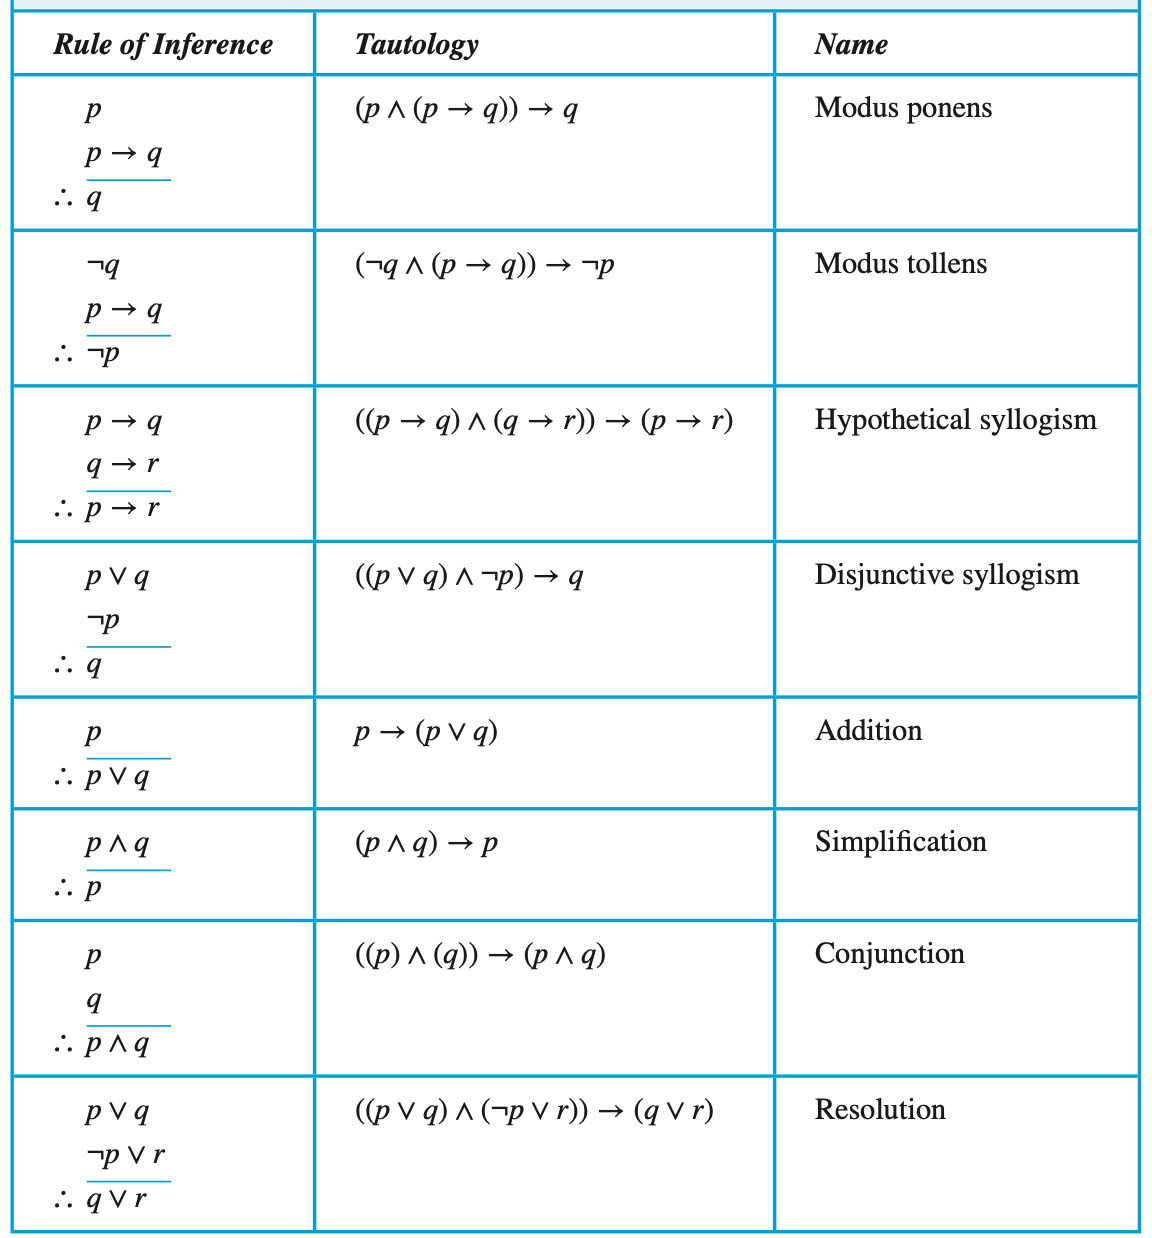
\includegraphics[scale = 0.5]{inference_1.png}
    \\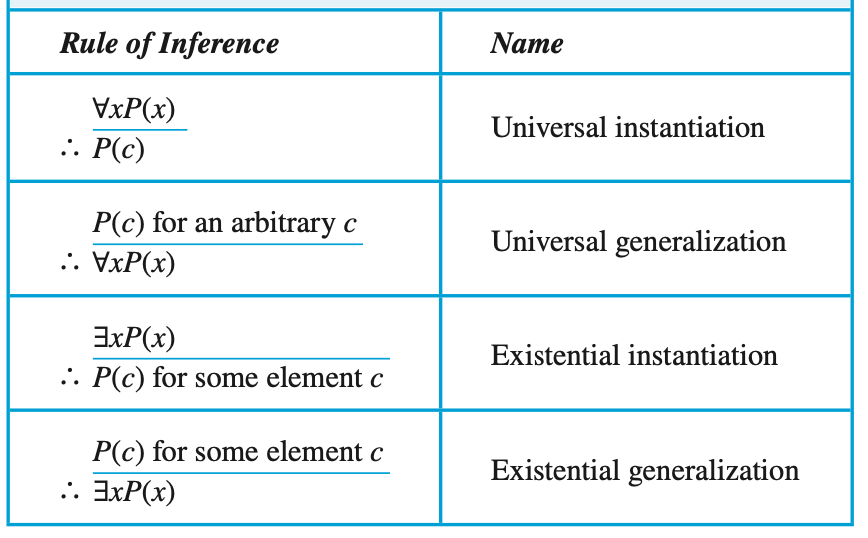
\includegraphics[scale = 0.66]{inference_2.png}
    \\Figure 1: Table of rules of inference. The tables are taken from Discrete Mathematics and Its Applications by Kenneth H. Rosen \cite{Rosen19}.
\end{center}

\subsubsection*{Problems}
\begin{questions}
    \question You're a bizarre adventure with Johnny Joestar to stop the president of the United States. You need to find pieces of the corpse of a saint.
    The adventure leads you to an island inhabited by knights, who always tell the truth, and knaves, who always lie. 
    Gyro Zeppeli tells you that a piece is in a cave. The cave is guarded by two enemy stand users $A$ and $B$, who are inhabitants of the island (they are either knights or knaves).
    They will only let you into the cave if you can determine, if possible, what $A$ and $B$ are if they address you in the ways described.
    % whether $A$ is a knight or a knave and if $B$ is a knight or a knave.
    % Determine, if possible, what $A$ and $B$ are if they address you in the ways described.
    \begin{parts}
        \part $A$ says ``At least one of us is a knave'' and $B$ says nothing.
        \begin{solution}
            If $A$ is a knave, then they are telling the truth as there does indeed exist at least one knave. But knaves always lie, so $A$ cannot be a knave. 
            Then $A$ is a knight. Knights always tell the truth, therefore, there must indeed be a knave among the two. $A$ cannot be a knave, therefore $B$ is a knave.
        \end{solution}

        \part $A$ says ``The two of us are both knights'' and $B$ says ``$A$ is a knave''.
        \begin{solution}
            If $A$ is a knight, then $A$'s statement must be true. However, $B$'s statement contradicts $A$'s statement. So $B$ cannot be a knight, and this case is false. 
            However, if $B$ is a knave, then $B$ is telling a lie, which contradicts $A$'s statement, therefore, $A$'s statement cannot be true. So this case is false.
            If $A$ is a knave, and $B$ is a knave, then $B$ is telling the truth, so this can't be the case. 
            Then if $A$ is a knave, and $B$ is a knight, there is no contradiction here, as $A$ is telling a lie which holds as a knave must always tell lies, and $B$ is telling the truth that $A$ is a knave. 
            Therefore, $A$ is a knave and $B$ is a knight.
        \end{solution}

        \part $A$ says ``I am a knave or $B$ is a knight'' and $B$ says nothing.
        \begin{solution}
            If $A$ is a knave, then he is telling the truth about himself, that he is a knave which implies his statement is true. 
            But knaves always lie, so his statement should be false, therefore $A$ cannot be a knave. Then $A$ is a knight.
            Now we know that $A$ is a knight, so $A$'s statement, ``I am a knave'' is not true, so for the statement to be true, ``B is a knight'' must be true. 
            \\Then it can be concluded that $A$ is a knight, and $B$ is a knight.
        \end{solution}

        \part Both $A$ and $B$ say ``I am a knight''
        \begin{solution}
            It cannot be determined as both statements can hold in either scenario. If A is a knight, he is telling the truth so is true, but if $A$ is not a knight, he is lying which means he is a knave, which is also true. 
            \\The same argument holds for $B$, therefore $A$ and $B$ cannot be determined.
        \end{solution}

        \part $A$ says we ``We are both knaves '' and $B$ says nothing.
        \begin{solution}
            If $A$ is a knight, then this statement is false by the rules of the knight, therefore $A$ is not a knight. So $A$ must be a knave. 
            $A$ is a knave, then $A$'s statement must be a lie and both cannot be knaves. Since $A$ is a knave, then $B$ cannot be a knave so $B$ is a knight. 
            $A$ is a knave and $B$ is a knight. 
        \end{solution}
    \end{parts}

    \question Three Vulcans walk into the mess hall of the starship enterprise. Spock approaches them with a cake and asks ``Does everyone want some cake?''
    The first Vulcan says ``I don't know''. The second Vulcan says ``I don't know''. Finally, the third Vulcan says ``No''. 
    Spock comes back and gives slices of cake to the Vulcan who wanted cake. How did Spock figure out who wanted the cake? (The Vulcans are a humanoid species from the planet Vulcan. They are widely renowned for their strict adherence to logic and reason as well as their remarkable stoicism. Spock is also a Vulcan.)

    \question 
    Professor Paradox has been taken captive by Eon. In order to save him you need to find his Chrononavigator which he hid somewhere.
    Lucky for you, he left clues behind to find the Chrononavigator. By using the following clues deduce where the Chrononavigator is hidden.
    \begin{itemize}
        \item If Mr.Smoothy is next to a Burger Shack, then the Chrononavigator is in the Plumber's headquarters.
        \item If Mr.Smoothy is not next to a Burger Shack or the Chrononavigator is buried under Baumann's Store, then the tree in the front of Billion Tower is an elm and the tree in the back of Billion Tower is not an oak.
        \item If the Chrononavigator is in the Argistix Security office, then the tree in the back of Billion Tower is not an oak.
        \item If the Chrononavigator is not buried under Baumann's Store, then the tree in front of Billion Tower is not an elm.
        \item The Chrononavigator is not in the Plumber's headquarters.
    \end{itemize}
   
    % \begin{itemize}
    %     \item If the house is next to a lake, then the treasure is in the kitchen.
    %     \item If the house is not next to a lake or the treasure is buried under the flagpole, then the tree in the front yard is an elm and the tree in the back yard is not an oak.
    %     \item If the treasure is in the garage, then the tree in the backyard is not an oak.
    %     \item If the treasure is not buried under the flagpole, then the tree in the front yard is not an elm.
    %     \item The treasure is not in the kitchen.
    % \end{itemize}
    Using rules of inference, determine where the Chrononavigator is hidden. Clearly state what your propositions
    represent.
    \begin{solution}
        % Our propositions are as follows: \\ 
        % $p$: ``The house is next to a lake'' \\ 
        % $q$: ``The treasure is in the kitchen'' \\ 
        % $r$: ``The treasure is buried under the flagpole'' \\ 
        % $s$: ``The tree in the front yard is an elm'' \\ 
        % $t$: ``The tree in the back yard is an oak'' \\ 
        % $u$: ``The treasure is in the garage'' 

        % The above situation in propositional logic can be represented as: \\ 
        % 1: $ p \implies q $ \\ 
        % 2: $ (\neg p \lor r) \implies (s \land \neg t) $ \\ 
        % 3: $ u \implies \neg t $ \\ 
        % 4: $ \neg r \implies \neg s $ \\ 
        % 5: $ \neg q $
        
        % \vspace{2mm}
        % Now we know that $ \neg q $ is true. \\ 
        % Then $ \neg q \implies \neg p $ (By Contrapositive) \\ 
        % So $ \neg p $ is true by Modus Tollens.
        
        % Then: $ (\neg p \lor r) $ is true. \\ 
        % $ \therefore s \land \neg t $ is true. \\ 
        % $ \therefore s $ is true by Simplification \\ 
        % $ \therefore \neg t $ is true by Simplification 

        % Then by taking the contrapositive of proposition 4 \\ 
        % $ s \implies r $ [A conditional statement has the same truth value as its contrapositive] \\ 
        % Since $s \implies r$, and we know $s$ is true, therefore $r$ is true by Modus Ponens. 

        % Hence we can conclude that the treasure is buried under the flagpole.
    \end{solution}

    \question Show that the following are logically equivalent without using truth tables
    \begin{parts}
        \part $ (p \implies r) \lor (q \implies r)  \equiv  (p \land q) \implies r $
        \begin{solution}
            $ (p \implies r) \lor (q \implies r)  \equiv  (p \land q) \implies r $ \\ 
            LHS: \\ 
            $ \neg((p \implies r) \lor \neg(q \implies r)) $ \hspace{10mm} {\color{red} [$ \neg (A \lor B) \equiv \neg A \land \neg B $]}\\ 
            $ (p \land \neg r) \land (q \land \neg r) $ \hspace{21.5mm} {\color{red} [$ \neg (p \implies q) \equiv p \land \neg q $]}\\ 
            $ (p \land q) \land \neg r $ \hspace{31mm} { \color{red} [Distributive Law]}\\ 
            $ (p \land q) \implies r $ \hspace{27.5mm} { \color{red} [$ \neg (p\implies q) \equiv p \land \neg q $]} \\ 
            RHS: \\ 
            $ \neg ((p \land q) \implies r) $ \\ 
            $ (p \land q) \land \neg r $ \\ 
            $ (p \land \neg r) \land (q \land \neg r) $ \\ 
            $ \neg ((p \land \neg r) \land (q \land \neg r)) $ \\ 
            $ \neg (p \land \neg r) \lor \neg(q \land \neg r) $ \\ 
            $ \neg \neg (p \implies r) \lor \neg \neg (q \implies r) $ \\ 
            $ (p \implies r) \lor (q \implies r) $ 
        \end{solution}
        \part $ p \land (q \lor r) \equiv (p \land q) \lor (p \land) r $
        \part $ \neg [\neg[(p \lor q) \land r] \lor \neg q] \equiv q \land r $
        \part $ (p \lor q \lor r) \land (p \lor t \lor \neg q) \land (p \lor \neg t \lor r) \equiv p \lor [r \land (t \lor \neg q)] $
    \end{parts}

\end{questions}

% \subsection*{Boolean formula}
% A boolean variable is a variable let's say $x$ which can have two values either \emph{true} or \emph{false}.
% A literal 


\section*{Proofs}
When we talk about mathematical statements we need to ``prove'' their validity. If I make a mathematical assertion I need to be able to show that the assertion is indeed true.
A proof is a valid argument that establishes the truth of a mathematical statement. 
A theorem is a statement that is proved to be true. In mathematics, by theorems, we generally refer to statements that are of some importance. Less important statements are often called propositions.
Axioms are statements that we assume to be true, these come from how we define things, or from our observation of intuition about the world. For example, an axiom can be that ``two sets are equal if they have the same elements'' (this is known as the Axiom of extensionality in Zermelo-Fraenkel set theory).
A less important theorem that is helpful in the proof of other results is called a lemma. A corollary is a theorem that can be established directly from a theorem that has been proved. A conjecture is a statement that is being proposed to be a true statement, but we don't have a proof yet.
Now we look at some proof techniques. These are general ideas our proofs usually follow. In writing a proof we have to be creative, we don't have a method or an algorithm to construct a proof for any statement, so we need to be very creative with our arguments.
Ideally, a mathematical proof should be elegant and concise, the more simple and short the argument for a complex theorem the more beautiful the proof is.

\subsection*{Direct Proof}
The first proof technique we look at is direct proof. Direct proofs are pretty straightforward.
A direct proof shows that a conditional statement $p \implies q$ is true by showing that if $p$ is true, then $q$ must also be true so that the combination $p$ true and $q$ false never occurs. We do this by assuming that $p$ is true and use axioms, definitions, and previously proven theorems, together with rules of inference, to show that $q$ must also be true.

We will now look at an example of a direct proof.
\begin{theorem}
    If $n$ is an odd integer, then $n^2$ is odd.
\end{theorem}
\begin{proof}
    Let $n$ be an odd integer, then there exists an integer $k$ such that $n = 2k+1$ (an odd integer is always of form $n = 2k+1$).
    Then $n^2 = (2k+1)^2 =  4k^2 + 2k + 1 = 2(2k^2 + k) + 1$, therefore $n^2$ is also odd.
\end{proof}



\subsection*{Contrapositive}
Often we are unable to prove a statement by direct proof, and for that, we might sometimes use another proof technique called proof by contradiction.
Proofs by contraposition make use of the fact that $p \implies q$ is equivalent to its contrapositive, $\neq q \implies \neg p$. 
This means that $p \implies q$ can be proved by showing that its contrapositive, $\neq q \implies \neg p$, is true. 
In a proof by contraposition of $p \implies q$, we take $\neg q$ as a premise, and using axioms, definitions, and previously proven theorems, together with rules of inference, we show that $\neg p$ must follow. 
We will now look at an example of a proof by contrapositive.

\begin{theorem}
    If $x^{2} - 6x + 5$ is even, then $x$ is odd.
\end{theorem}
\begin{proof}
    Let $p$ be `$x^2 - 6x + 5$ is even' and let $q$ be `$x$ is odd'.
    Then by the statement $ p \implies q $ the contrapositive is, $ \neg q \implies \neg p $.
    Therefore, if $x$ is even, $x^2 -6x + 5 $ is odd.
    Then $x$ can be represented as $x = 2k$ where $k \in \mathbb{Z} $.
    Then $x^2 - 6x + 5 = (2k)^2 - 6(2k) + 5 = 4k^2 -12k + 5  = 2(2k^2 - 6k) + 5 =2\alpha + 5$ where $ \alpha = 2k^2 - 6k$. 
    Then $ 2\alpha $ is also an even number as it is of the form $ 2k $, and since the sum of an even number and an odd number is odd (5 is odd), therefore, the result is odd. 
\end{proof}
 

\subsection*{Contradiction}
Often even a proof by contrapositive doesn't work, and we are unsuccessful in proving a statement by contrapositive, in that case, we may also try a proof by contradiction approach.
Suppose we want to prove that a statement $p$ is true. 
Furthermore, suppose that we can find a contradiction $q$ such that $\neg p \implies q$ is true. 
Because $q$ is false, but $\neg p \implies q$ is true, we can conclude that $\neg p$ is false, which means that $p$ is true.
This type of proof is called a proof by contradiction.
We will now look at an example of a proof by contradiction.
\begin{theorem}
    Show that $\sqrt{2}$ is an irrational number.
\end{theorem}
\begin{proof}
    We want to reach a contradiction, and for that, we suppose that the negation of our statement is true.
    So suppose $\sqrt{2}$ is a rational number. Let $\sqrt{2} = \frac{p}{q}$ for some integers $p$ and $q$ such that $q \neq 0$, also suppose that $\frac{p}{q}$ is in the in lowest terms so $\gcd(p,q) = 1$.
    Then $2 = \frac{p^2}{q^2} \iff 2q^2 = p^2$ which implies $p^2$ is even, and therefore $p$ is even.
    As $p$ is even there exists an integer $k$ such that $p = 2k$.
    So $2 = \frac{p^2}{q^2} = \frac{(2k)^2}{q^2} \iff q^2 = \frac{4k^2}{2} = 2k^2$, which implies that $q^2$ is even and so $q$ is even. But if $p$ and $q$ are both even then $\frac{p}{q}$ is not in lowest terms as then $2 | p$ and $2|q$ and so $\gcd(p,q) \geq 2$, which is a contradiction as we have that $\gcd(p,q) = 1$.
    Therefore $\sqrt{2}$ cannot be written in the form $\frac{p}{q}$, and so $\sqrt{2}$ is not rational and therefore $\sqrt{2}$ is irrational.
\end{proof}

\subsection*{Induction}
Now we look at another proof technique, called proof by induction. This technique is a bit different from the other proof techniques we have seen so far.
Proof by induction uses the principle of mathematical induction. The principle of mathematical induction is used to prove properties regarding the set of natural numbers (or a subset of it) the principle can be generalized to apply to any wellfounded set but at this level, we need not be concerned about that.
The principle of mathematical induction is defined as follows, suppose we want to prove $P(n)$ is true for all positive integers $n$, where $P(n)$ is a propositional function, then if we show that $P(1)$ is true (this is called the base case), and for any positive integer $k$, $P(k) \implies P(k+1)$ (this is called the induction step), then we can conclude that $P(k)$ holds for all positive integers.
We can think of this like a series of dominoes, if the first domino falls and we have that if any $k^{\text{th}}$ domino falling means that $k+1$ domino will also fall then we have that all the dominoes will fall.
Now we show an example of proof by induction.
\begin{theorem}
    For any positive integer $n$, the sum $1 + 2 + \dots + n = \sum\limits_{i = 1}^{n} i = \frac{n(n+1)}{2}$.
\end{theorem}
\begin{proof}
    By mathematical induction, we show that for any positive integer $n$, $\sum\limits_{i = 1}^{n} i = \frac{n(n+1)}{2}$ holds true.
    \\\textbf{Base case:} $n = 1$
    \\For $n = 1$ we have that $\sum\limits_{i = 1}^{1} i = 1$ and $\frac{1 (1+1)}{2} = 1$ so this case holds true.
    \\\textbf{Induction hypothesis:} Suppose that $n = k$, $\sum\limits_{i = 1}^{k} i = \frac{k(k+1)}{2}$ is true.
    \\\textbf{Induction step:} We use our induction hypothesis to show that $P(k) \implies P(k+1)$.
    \\For $n = k+1$, we want to show that $\sum\limits_{i = 1}^{k+1} i = \frac{(k+1)((k+1)+1)}{2}$.
    We have that $\sum\limits_{i = 1}^{k+1} i = \left(\sum\limits_{i = 1}^{k} i\right) + k+1$. From our induction hypothesis, we have that $\sum\limits_{i = 1}^{k} i = \frac{k(k+1)}{2}$, so
    $$\sum\limits_{i = 1}^{k+1} i = \left(\sum\limits_{i = 1}^{k} i\right) + k+1 = \frac{k(k+1)}{2} + k+1 = \frac{k(k+1) + 2(k+1)}{2} = \frac{(k+1)(k + 2)}{2} = \frac{(k+1)((k + 1)+1)}{2}$$
    And as $P(k) \implies P(k+1)$, we have that by the principle of mathematical induction for any positive integer $n$, the sum $1 + 2 + \dots + n = \sum\limits_{i = 1}^{n} i = \frac{n(n+1)}{2}$.
\end{proof}



\subsection*{Problems}
\begin{questions}
    \question Give a direct proof that if $m$ and $n$ are both perfect squares, then $nm$ is also a perfect square.
    \begin{solution}
        Let $n$ and $m$ be perfect squares, then there exists integer $a$ and $b$ such that $n = a^2$ and $m = b^2$.
        So $nm = a^2 b^2 = (aa)(bb) = (ab)(ab) = (ab)^2$. Therefore $nm$ is also a perfect square.
        \\\qed
    \end{solution}

    \question Given that $p$ is a prime and $p|a^n$, prove that $p^n|a^n$. 
    \begin{solution}
            As $p|a^n$ then $a^n = kp$ for some integer $k$.
            \\\textbf{Case 1:} $p \neq a$
            \\Then $a$ is not a prime, then $a = p_1\times p_2 \times ... p_m$
            \\$a^n = p_1^n\times p_2^n \times ... p_m^n = kp$
            \\As $p|a^n$ and $a^n = p_1^n\times p_2^n \times ... p_m^n$ then there must be some $p_i$ from $1\leq i \leq m$ such that $p|p_i$
            \\As $p_i$ is prime for all $i \leq i \leq m$, then if $p|p_i$ then $p_i = p$ which means $p|a$
            \\Then $a = pq$ so $a^n = p^n q^n$ therefore $p^n|a^n$.
            \\\textbf{Case 2:} $p = a$ 
            \\If $p = a$  and $p|a^n$ then as $a^n|a^n$ and $a^n=p^n$ then $p^n|a^n$.
        \\\qed
    \end{solution}

    \question Show that any composite three-digit number must have a prime factor less than or equal to 31.
    \begin{solution}
        The largest composite three-digit number is 999.
        Any composite number can be expressed as the product of two or more primes. For a three-digit composite number, the primes must be at most the square root of the number. Therefore, to show that any composite three-digit number must have a prime factor less than or equal to 31, it suffices to show that there are no primes greater than 31 that divide any of the numbers from 100 to 999.
        Then $ 31^2 = 961 $ which is less than 999. Henceforth it suffices. 
        Then any three-digit number that is divisible by a prime greater than 31 would have to be divisible by the next prime number which is 37. $ 37^2 = 1369 $ which is a 4-digit composite number. Hence shown.
        \\\qed
    \end{solution}

    \question Show that if $a$ is a positive integer and $\sqrt[n]{a}$ is rational, then $\sqrt[n]{a}$ must be an integer.
    \begin{solution}
        Let $a \in \mathbb{Z}^+$, suppose $\sqrt[n]{a}$ is rational, we show that then $\sqrt[n]{a}$ must be an integer.
        \\Let $\sqrt[n]{a} = \frac{p}{q}$, where $p,q \in \mathbb{Z}$ where $q \neq 0$ and $\text{gcd}(p,q) = 1$.
        $$\sqrt[n]{a} = \frac{p}{q} \Leftrightarrow a = \frac{p^n}{q^n} \Leftrightarrow a q^n = p^n$$
        Now we have that $q^n | p^n$, but as $\text{gcd}(p,q) = 1$ then $\text{gcd}(p^n,q^n) = 1$.
        \\So as only common divider of $p^n$ and $q^n$ is 1 and $q^n | p^n$ then $q^n = 1$
        \\Therefore $ a = \frac{p^n}{q^n} = p^n$, so $\sqrt[n]{a} = p$.
        \\Which means $\sqrt[n]{a}$ is an integer.
        \\\qed
    \end{solution}

    \question Show that there exists irrational numbers $a$ and $b$ such that $a^b$ is rational.
    \begin{solution}
        It is enough to prove this claim through an example that there exist rational numbers $a$ and $b$ such that $a^b$ is rational. 

        Consider $a = \sqrt{2}$ and $ b = \sqrt{2} $. Then a number $ c = a^b = \sqrt{2}^{\sqrt{2}} $ where $ c \in \mathbb{R} $

        Then either $ c $ is rational, or $c$ is irrational. 

        \textbf{Case 1:} $c$ is rational. \\ 
        If $ c = \sqrt{2}^{\sqrt{2}} $ is rational, then we already have our irrational numbers $a$ and $b$ such that $ a^b $ is rational.
            
        \textbf{Case 2:} $c$ is irrational. \\ 
        If $c = \sqrt{2}^{\sqrt{2}} $ is irrational, then let $ a = \sqrt{2}^{\sqrt{2}} $ and $ b = \sqrt{2} $. Then $$ c = \biggl( \sqrt{2}^{\sqrt{2}} \biggr)^{\sqrt{2}} = 2$$
        and 2 is rational.

        Hence proved that there exists irrational numbers $a$ and $b$ such that $ a^b $ is rational.
        \\\qed
    \end{solution}

    \question Show that there are infinitely many primes. You may like to use the following definition and theorem in your proof.
    \\ \textbf{Definition:} A prime number is a Natural number that is only divisible by 1 and itself and has to be divisible by 2 different numbers.
    \\\textbf{Fundamental Theorem of Arithmetic:} Every integer $N > 1$ has a prime factorization, meaning either $N$ is itself prime or can be written as a product of prime numbers.
    \begin{solution}
        Let $s=\{p_0,p_1,p_2,...,p_n\}$ be set of all primes. 
        \\Let $P = p_0 \times p_1 \times p_2 \times ... \times p_n$
        \\Let $q = P+1$
        \\\textbf{Case 1:}
        \\$q$ is prime, which is not in our set $s$
        \\\textbf{Case 2:} 
        \\if $q$ is not prime, then there exists a prime factor decomposition of $q$.
        \\Let $f$ be a prime that divides $q$, then $f$ would be in our set $s$ thus $f$ would divide $P$ too. 
        \\As $f$ divides $q$ and $P$ then $f$ divides $q-P$, which is $1$
        \\Then $f$ divides 1.
        \\As $f\geq2$ $f$ cannot divide 1, thus we have a contradiction.

        Hence, the new prime number $q$ does not exist in our set but lies outside the set. But we claimed that our set contains all prime numbers. Therefore, there are infinite prime numbers.
        \\\qed
    \end{solution}

    \question Show that for any positive integer $n$, $\sum\limits_{i = 1}^{n} 2i-1 = n^2$
    \question Show that for any natural number $n$, $\sum\limits_{i = 1}^{n} 2^i = 2^{n+1}-1$
    \question Prove that for all natural numbers $n>1$, $ \sqrt[n]{n}$ is irrational
    \begin{solution}
        Suppose $\sqrt[n]{n}$ is rational for some $n \in \mathbb{N}$
        \\Then there exists integers $a$ and $b$, such that $\sqrt[n]{n} = \frac{a}{b}$, where $b \neq 0$ and $gcd(a,b) =1$
        $$\sqrt[n]{n} = \frac{a}{b} \Rightarrow n = \frac{a^n}{b^n}$$
        $$gcd(a,b) =1 \Rightarrow gcd(a^n,b^n) =1$$
        As $n \in \mathbb{N}$, then $b^n = 1$, which means $n = a^n$
        \\As $n > 0$ and $b^n = 1$, then $a^n > 0$, which means that $a > 0$
        \\$a \neq 1$, as if $a = 1$ then $n = \frac{a^n}{b^n} = \frac{1}{1} = 1$, but $n > 1$, so $a \geq 2$
        \\We know for all natural numbers $n$ $2^n > n$ (this result is trivial and can be easily proved by mathematical induction).
        \\So $a^n \geq 2^n > n$, which means $n \neq a^n$, there we have a contradiction without original claim that $n = a^n$
        \\Therefore for all natural numbers $n>1$, $ \sqrt[n]{n}$ is irrational
        \\\qed
    \end{solution}

    \question Show that $\sqrt{p}$ is irrational for any prime number $p$.
    \begin{solution}
        Suppose $\sqrt{p}$ is rational then $\sqrt{p} = \frac{r}{q}$ where $q \neq 0$ and $gcd(q,r) = 1$
        \\Then $p = \frac{r^2}{q^2}$, so $pq^2 = r^2$
        \\Now as $r^2 = r \times r$ then any number in prime factorization of $r^2$ would appear an even number of times. 
        \\Similiary any number in prime factorization on $q^2$ appear and even number of times.
        \\So take $q^2 = p_1 \times p_2 \times... p_n \times p_1 \times p_2 \times... p_n$
        \\As $p|r^2$ and $q^2|r^2$ then $r^2 = p \times p_1 \times p_2 \times... p_n \times p_1 \times p_2 \times... p_n$
        \\Now $p$ is a number that appears in the prime factorization of $r^2$ an odd number of times.
        \\Here we have a contradiction, therefore $\sqrt{p}$ is irrational.
        \\\qed
    \end{solution}

    \question For all positive integers $a$ and $b$ show that $\text{gcd}(a,b) \text{lcm}(a,b)=ab$.
    \begin{solution}
        Let $d = \text{gcd}$ for $a,b \in \mathbb{Z}$. Then $\exists p,q \in \mathbb{Z}$ s.t. $a = pd$ and $b = qd$.
        \\Let $m = \frac{ab}{d}$ then $m = aq = pb$. Which means $a|m$ and $b|m$ which means $m$ is a common multiple of $a$ and $b$.
        \\Now we need to show that $m$ is indeed the least common multiple of $a$ and $b$.
        \\Let $c$ be a common multiple of $a$ and $b$, then $c = at = sb$.
        \\From bezout's lemma we know that $\exists x,y \in \mathbb{Z}$ s.t. $d = ax + by$.
        \\We show that $m|c$ which would imply that $m \leq c$.
        $$\frac{c}{m} =  \frac{cd}{ab} = \frac{c(ax + by)}{ab} = \frac{cax}{ab} + \frac{cby}{ab}$$
        $$\frac{cax}{ab} + \frac{cby}{ab} = \frac{cx}{b} + \frac{cy}{a} = \frac{c}{b}x + \frac{c}{a}y$$
        $$\frac{c}{m} = \frac{c}{b}x + \frac{c}{a}y = sx + ty$$
        As $s,x,t,y \in \mathbb{Z}$ then $sx + ty \in \mathbb{Z}$, which means $m|c$ theefore $m \leq c$.
        \\Which means $m$ is the least common multiple of $a$ and $b$.
        \\So we have that $dm = \text{gcd}(a,b) \text{lcm}(a,b) = ab$.
        \\\qed
    \end{solution}

    \question Prove that at a party where there are at least two people, there are two people who know the same number of other people there. Given that everyone at least knows the host.
    \begin{solution}
        Let there be $n$ number of people at the party where $n \in \mathbb{N}$ and $n\geq2$ 
        \\Now the maximum number of people a person can know is $n-1$
        \\The minimum number of people someone can know is 1 (the host).
        \\Now we have $n$ pigeons and $n-1$ holes, so with the pigeon hole principle at least 1 hole will have more than 1 pigeon. 
        \\So assigning the number of people that know that amount of people from 1 to $n-1$, there would be at least 1 number $k$ where 2 people are assigned.
        \\\qed
    \end{solution}
\end{questions}



\renewcommand\thefootnote{}


\renewcommand\thefootnote{\fnsymbol{footnote}}
\setcounter{footnote}{1}

\nocite*{}

\bibliographystyle{plain} 

\bibliography{resource.bib}


\end{document}




 


